\section{SceneNN 057: Observations and Object Map}
\begin{figure}[h!]
\centering
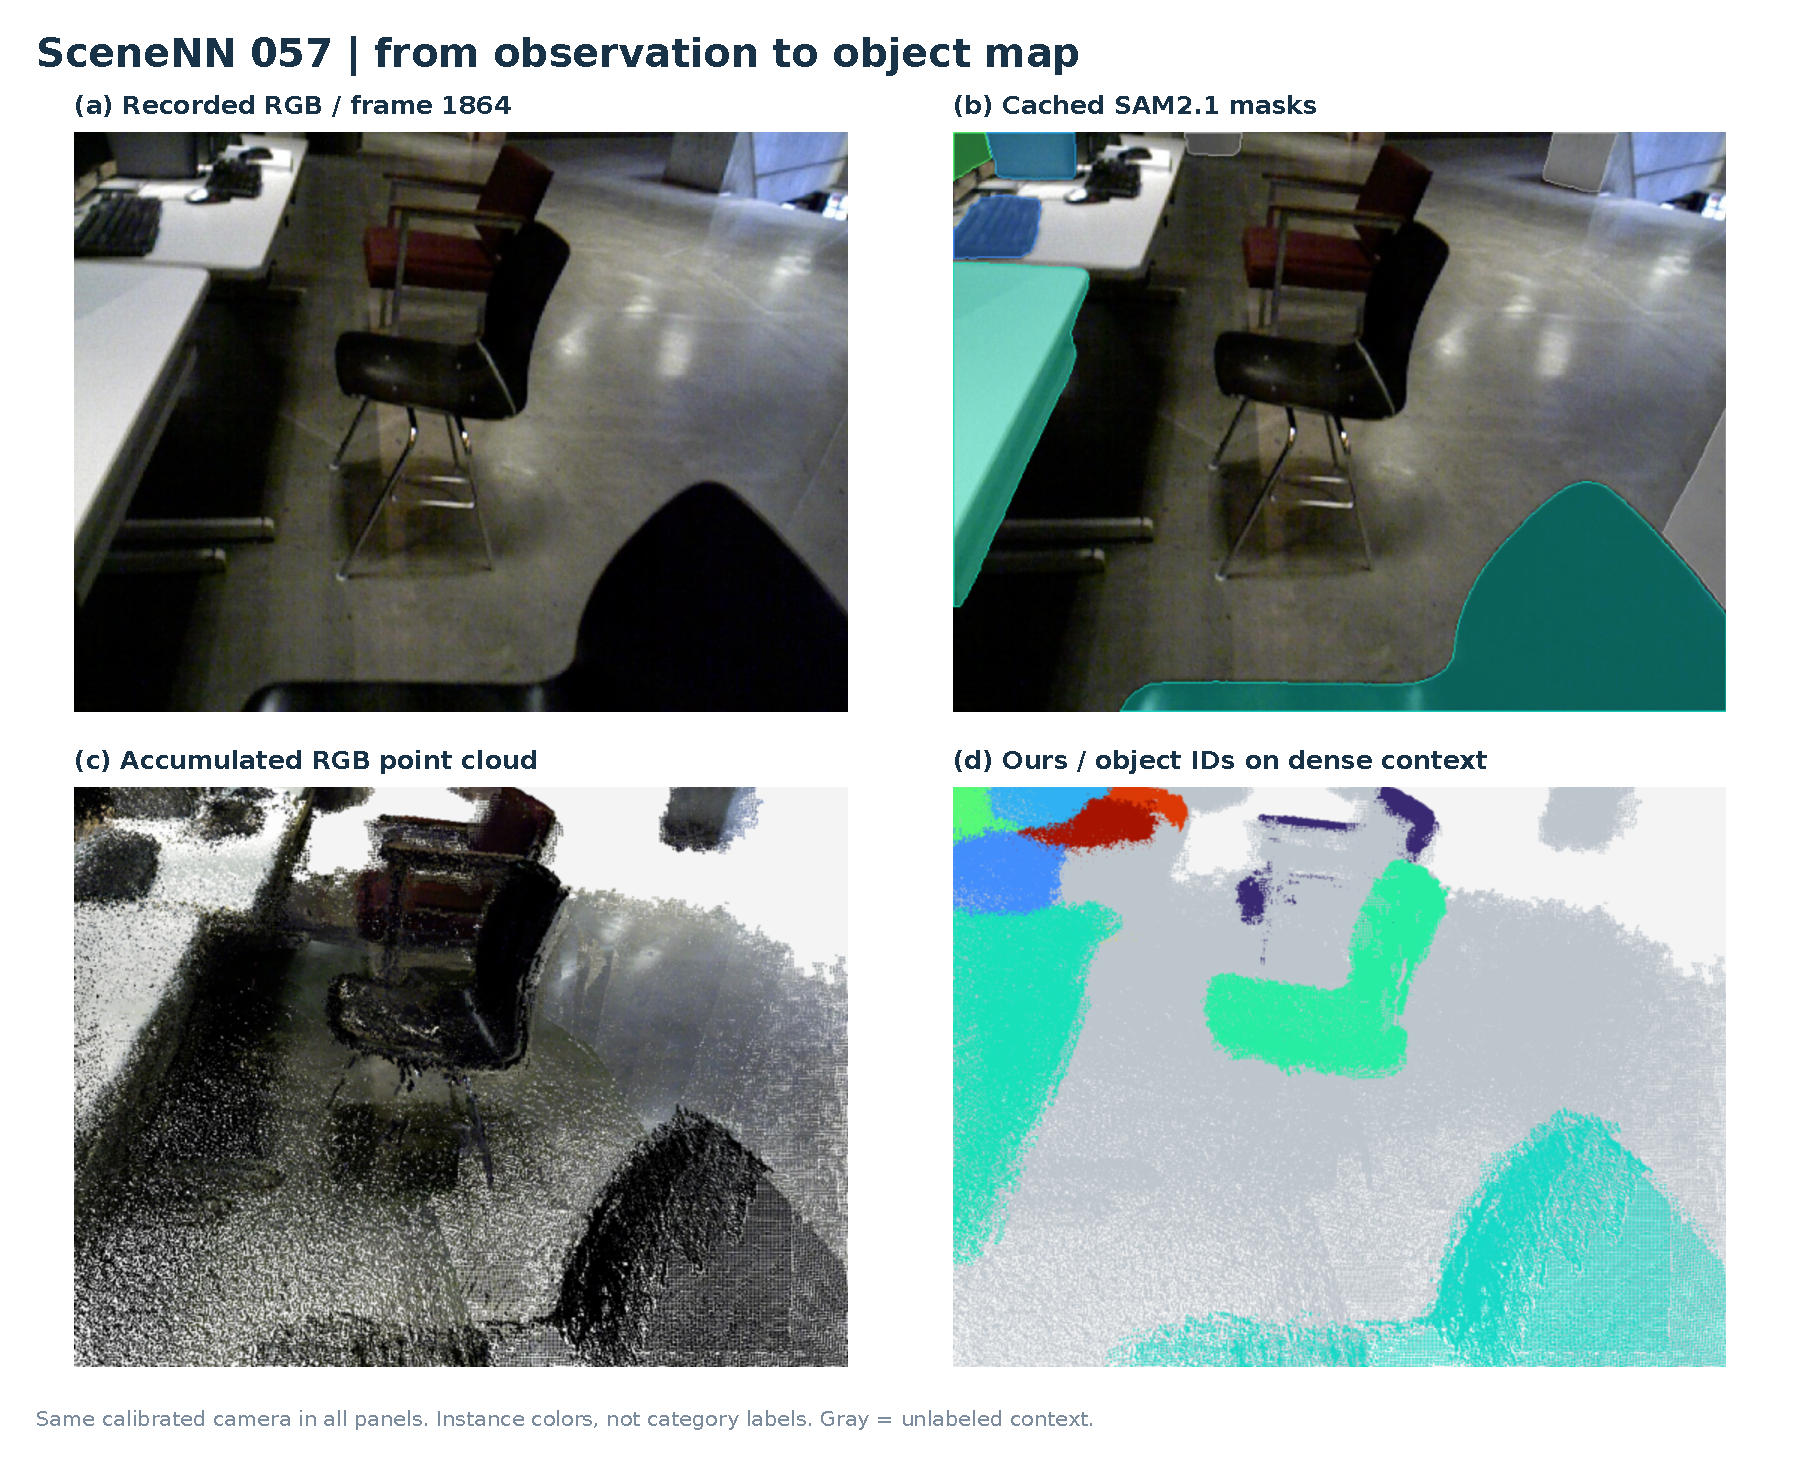
\includegraphics[width=.98\textwidth,height=.79\textheight,keepaspectratio]{dataset_scene_057.pdf}
\caption{Actual RGB, cached SAM2.1 masks, accumulated RGB cloud, and \ours{} instance map in the same calibrated camera. The frame was selected after evaluation to maximize support for explanatory predicted object 7. Point clouds use nearest-depth splats without hole completion. For dense context only, instance IDs are transferred within $3\,\mathrm{cm}$; gray indicates unlabeled context. Colors encode predicted identities, not ground-truth classes.}
\end{figure}
\clearpage

\section{SceneNN 061: A Second Evaluated Scene}
\begin{figure}[h!]
\centering
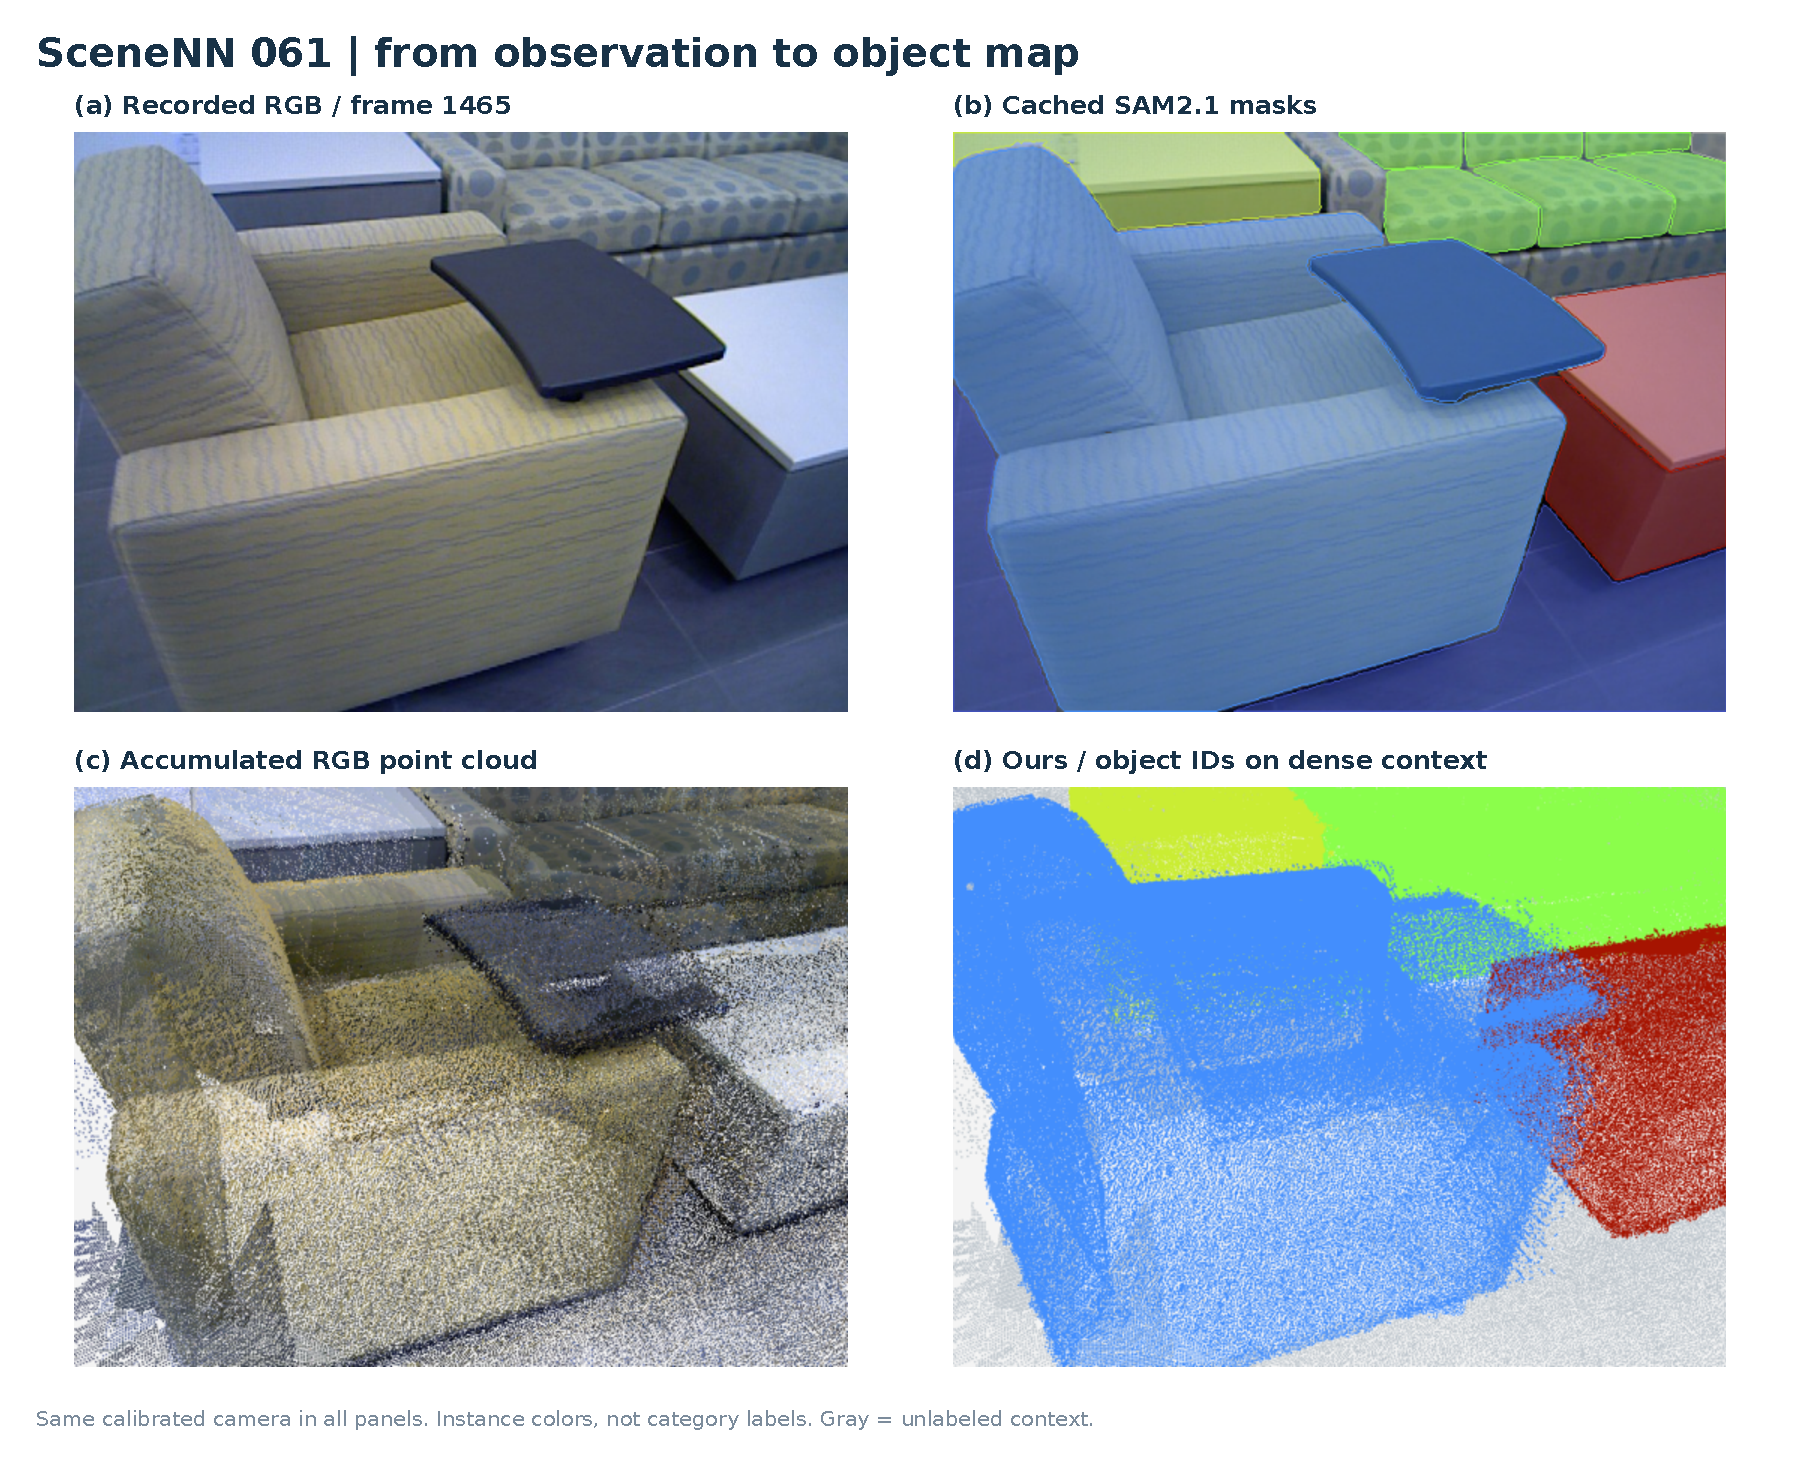
\includegraphics[width=.98\textwidth,height=.79\textheight,keepaspectratio]{dataset_scene_061.pdf}
\caption{Real RGB and segmentation of the seating area, accumulated colored geometry, and \ours{} object IDs. The same display rules as the preceding scene are used. The explanatory view maximizes cached support for predicted object 10. Accumulated geometry includes other viewpoints, so its coverage need not match the single image exactly.}
\end{figure}
\clearpage

\section{Garage: Object Locations and Supporting Observations}
\begin{figure}[h!]
\centering
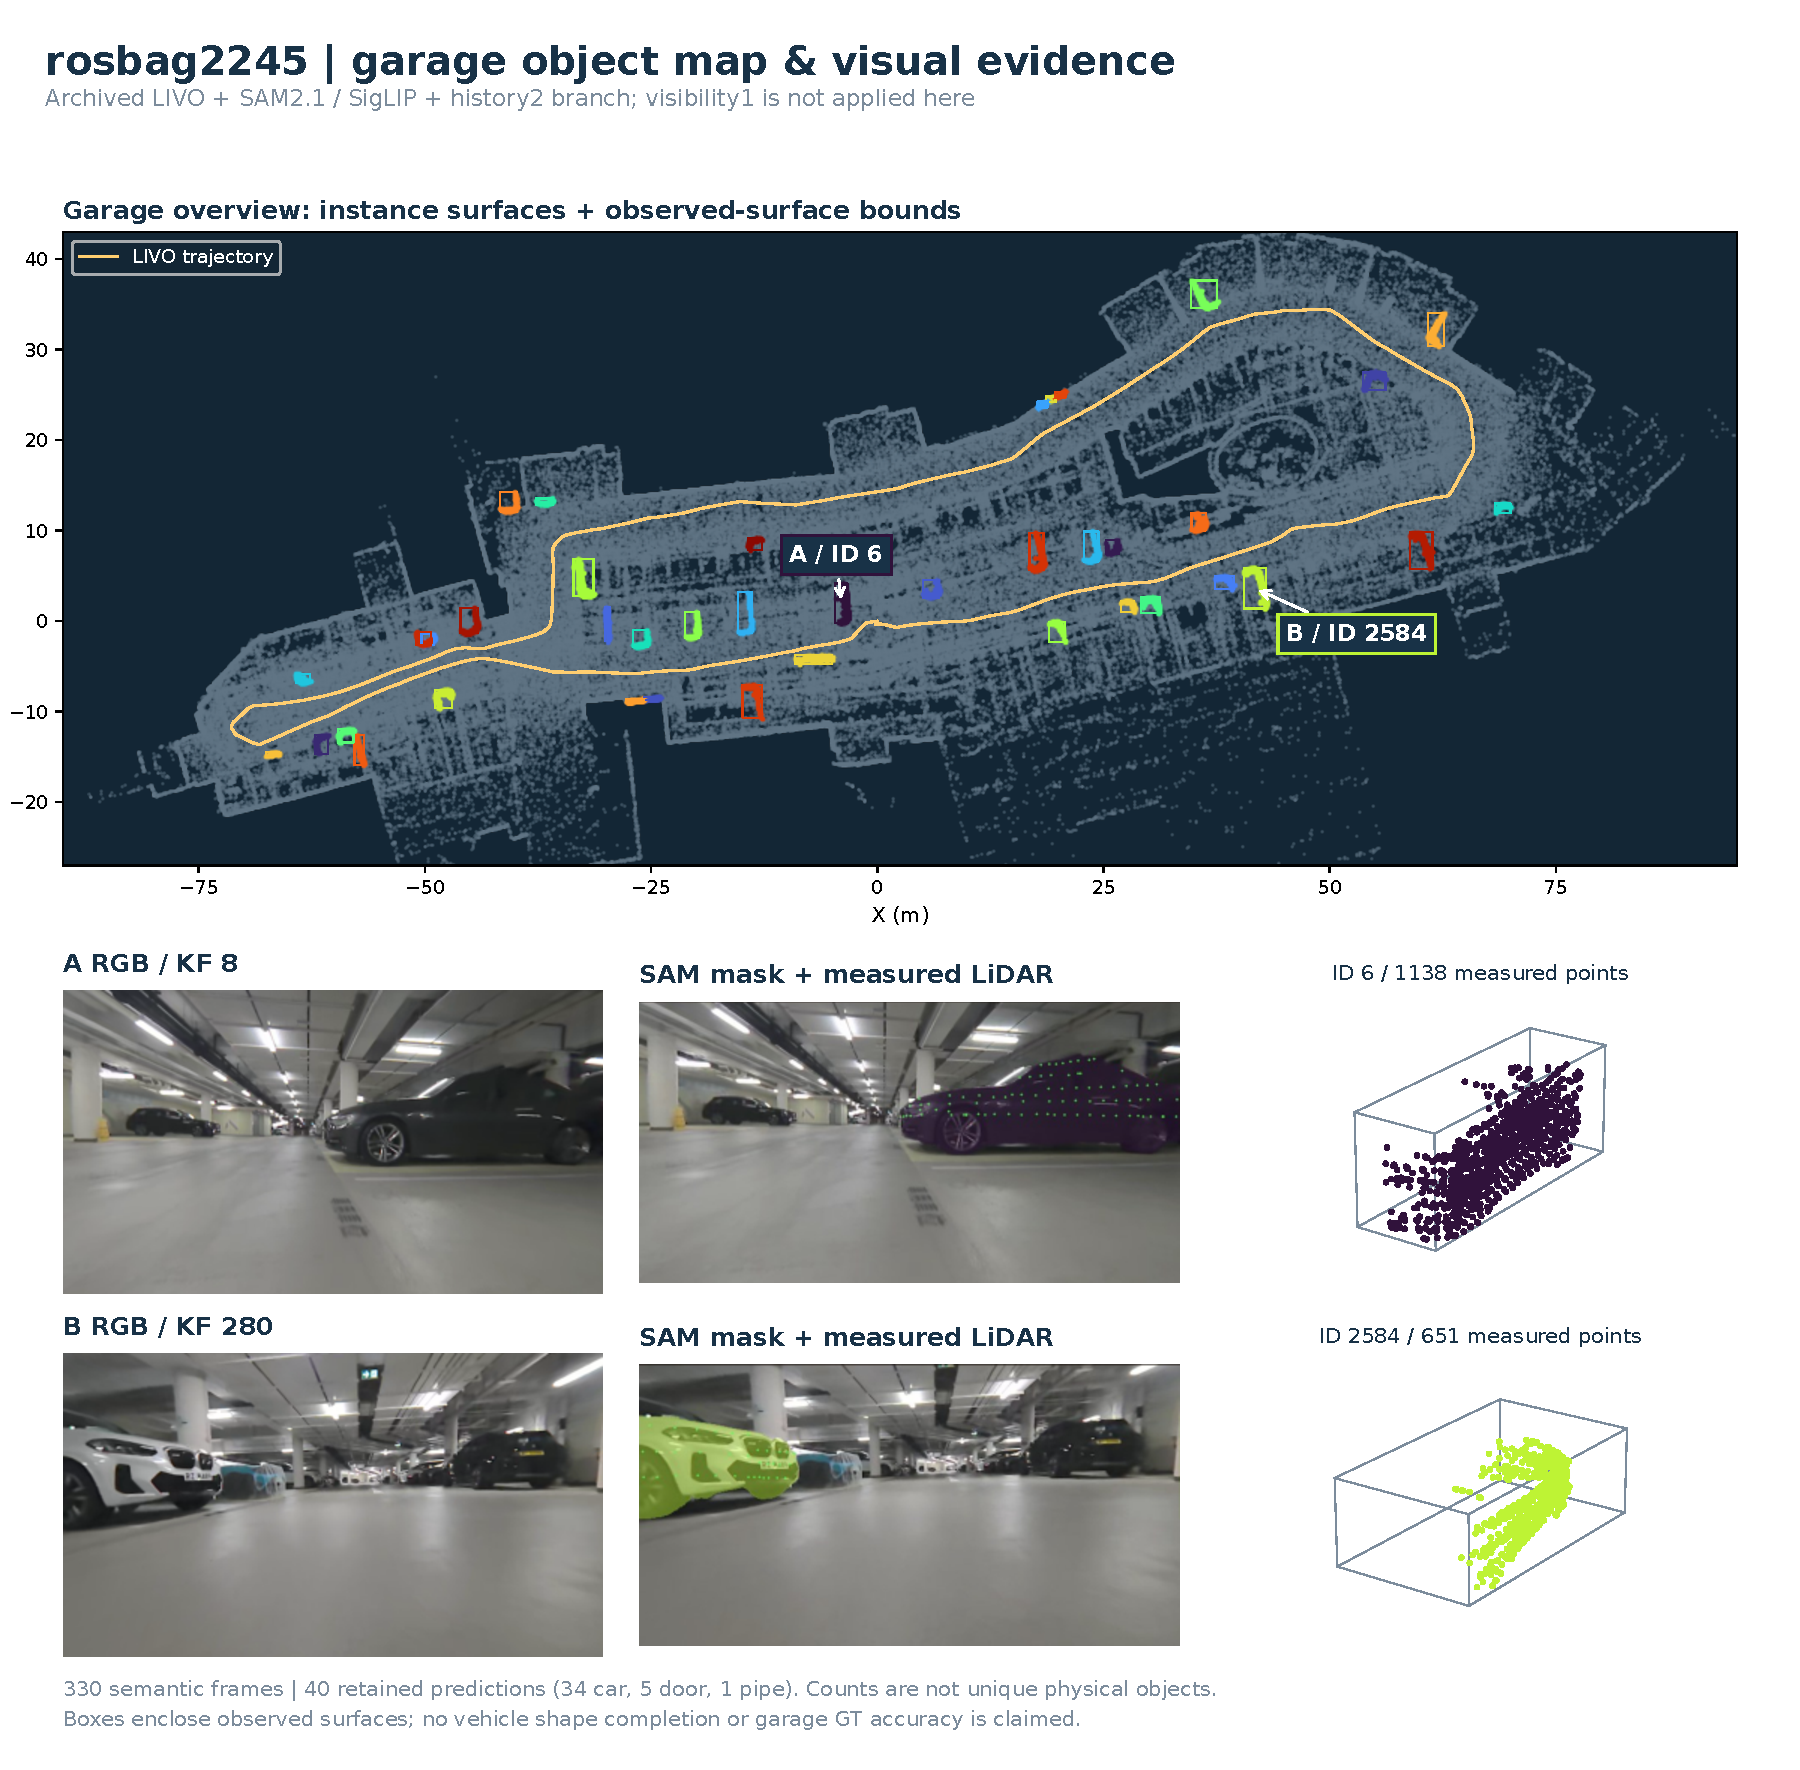
\includegraphics[width=.98\textwidth,height=.77\textheight,keepaspectratio]{garage_real_evidence.pdf}
\caption{Archived \texttt{rosbag2245} replay from the LIVO + SAM2.1/SigLIP + history2 branch. The map links vehicle records to actual RGB, masks, measured LiDAR support, and accumulated surfaces with bounding boxes. The overview shows all 40 retained predictions using a documented crop and context subsampling. The 330 cached semantic frames produce 34 car, five door, and one pipe records; these are not unique physical-object counts. Bounds enclose observed surfaces. The benchmark visibility1 module is not applied to this result.}
\end{figure}
\clearpage

\section{Six-Recording Inventory}
\begin{table}[h!]
\centering
\caption{Existing recordings and archived reviewed-map geometry. Path length is estimated from trajectories, not ground truth. Point counts refer to the full source maps before display subsampling.}
\begin{tabular}{lrrr}
\toprule
Recording & Minutes & Path (m) & Map points \\
\midrule
roabag2336 & 3.1 & 84.5 & 178,179 \\
rosbag0521\_2 & 4.0 & 108.8 & 199,568 \\
rosbag2245 & 9.8 & 316.2 & 565,791 \\
rosbag2\_20260415\_174148 & 18.9 & 556.9 & 2,148,498 \\
20260414\_4 & 24.3 & 838.4 & 2,778,455 \\
rosbag2\_20260415\_162852 & 27.4 & 834.9 & 3,063,285 \\
\bottomrule
\end{tabular}

\end{table}

The six recordings cover garage and outdoor routes and may revisit the same physical sites. They are not six independent semantic benchmark scenes. Raw files and corresponding maps are present in the working data repository. The following atlas pairs actual undistorted camera images with LIVO point clouds and trajectories from the reviewed offline backend. Point colors encode height, not camera RGB or semantic category. Displays use deterministic subsampling and the central 99\% XY extent, with a separate spatial scale for each recording.

The garage object-map page uses a later archived semantic branch and its original coordinate frame; the route atlas uses a separate reviewed map revision. The outdoor semantic and ground pages share their own internally consistent revision. No object overlay is transferred between these map versions.

The figures document qualitative engineering behavior without ground-truth trajectory or semantic accuracy. Static records require repeated observations; people remain transient observations. A three-dimensional box encloses measured surfaces and does not constitute an independently evaluated 3D detection or complete object-shape reconstruction.

\subsection{Model and Result Provenance}
The outdoor record \texttt{rosbag2\_20260415\_162852} contains 440 semantic keyframes. Grounding DINO tiny provides image detections, followed by measured-depth association. The archived static map retains 19 repeated-observation records (15 plant and four door/entrance candidates). SegFormer B0 with Cityscapes weights supplies ground candidates; local geometric checks determine the accepted LiDAR support. The original masks and detections are displayed without new inference.

The figure manifest records the source recording, selected frame or object, display transformation, source-map revision, and algorithm scope. No current visibility1 result is inferred from these archived branches. A real-robot comparison of the frozen revision module remains a separate evaluation task.
\clearpage

\section{Garage Route Atlas}
\begin{figure}[h!]
\centering
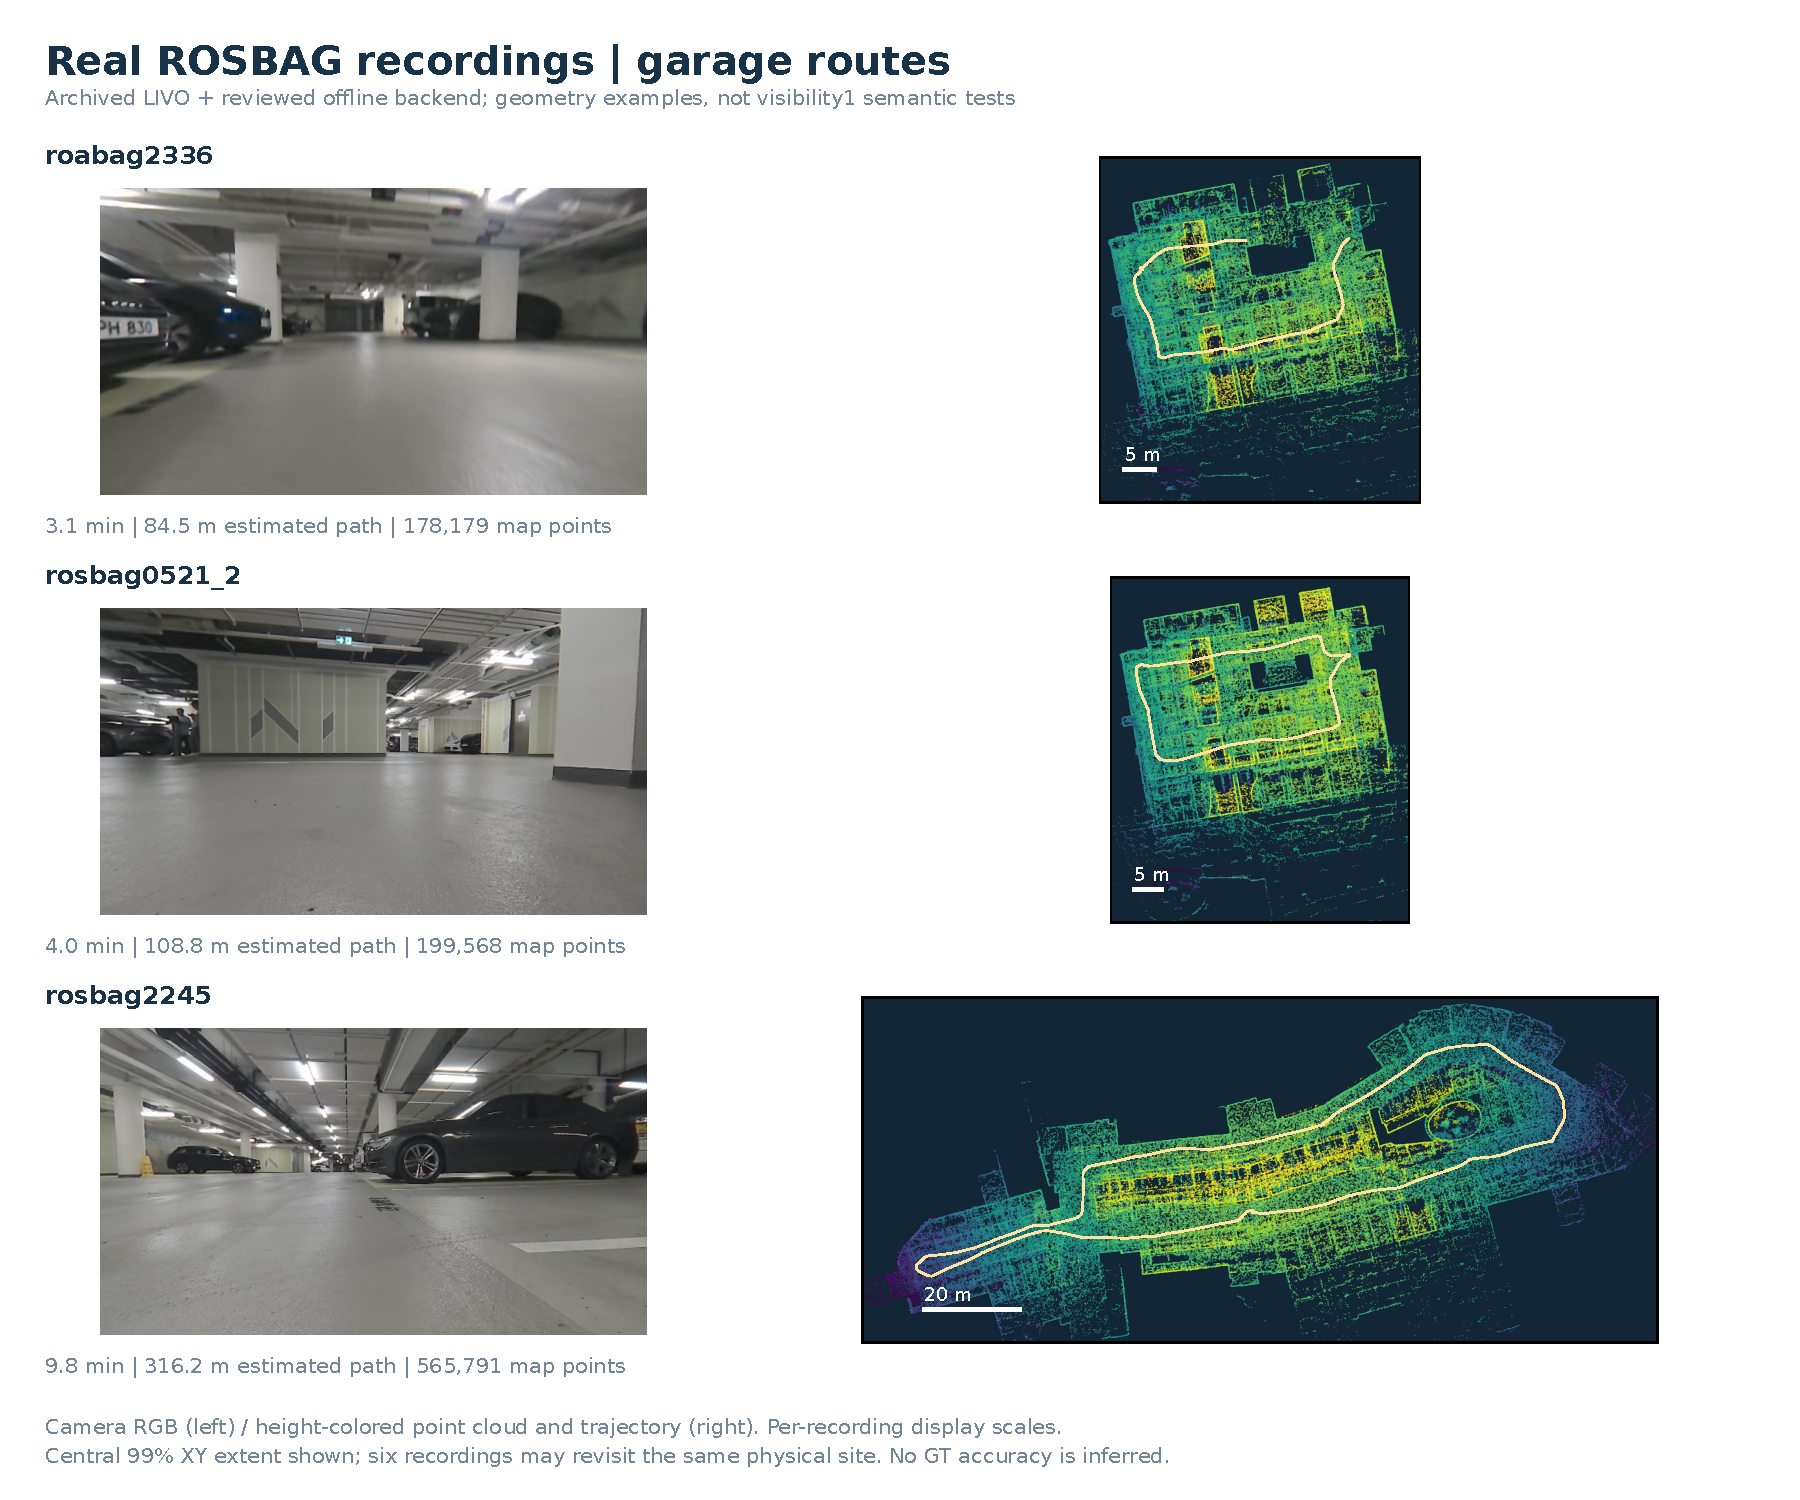
\includegraphics[width=.98\textwidth,height=.8\textheight,keepaspectratio]{rosbag_routes_1.pdf}
\caption{Three real garage recordings: camera views and height-colored point clouds with estimated trajectories. Per-recording map scales, durations, path lengths, and point counts are shown. These are archived LIVO geometry results, not three additional visibility1 tests.}
\end{figure}
\clearpage

\section{Outdoor Route Atlas}
\begin{figure}[h!]
\centering
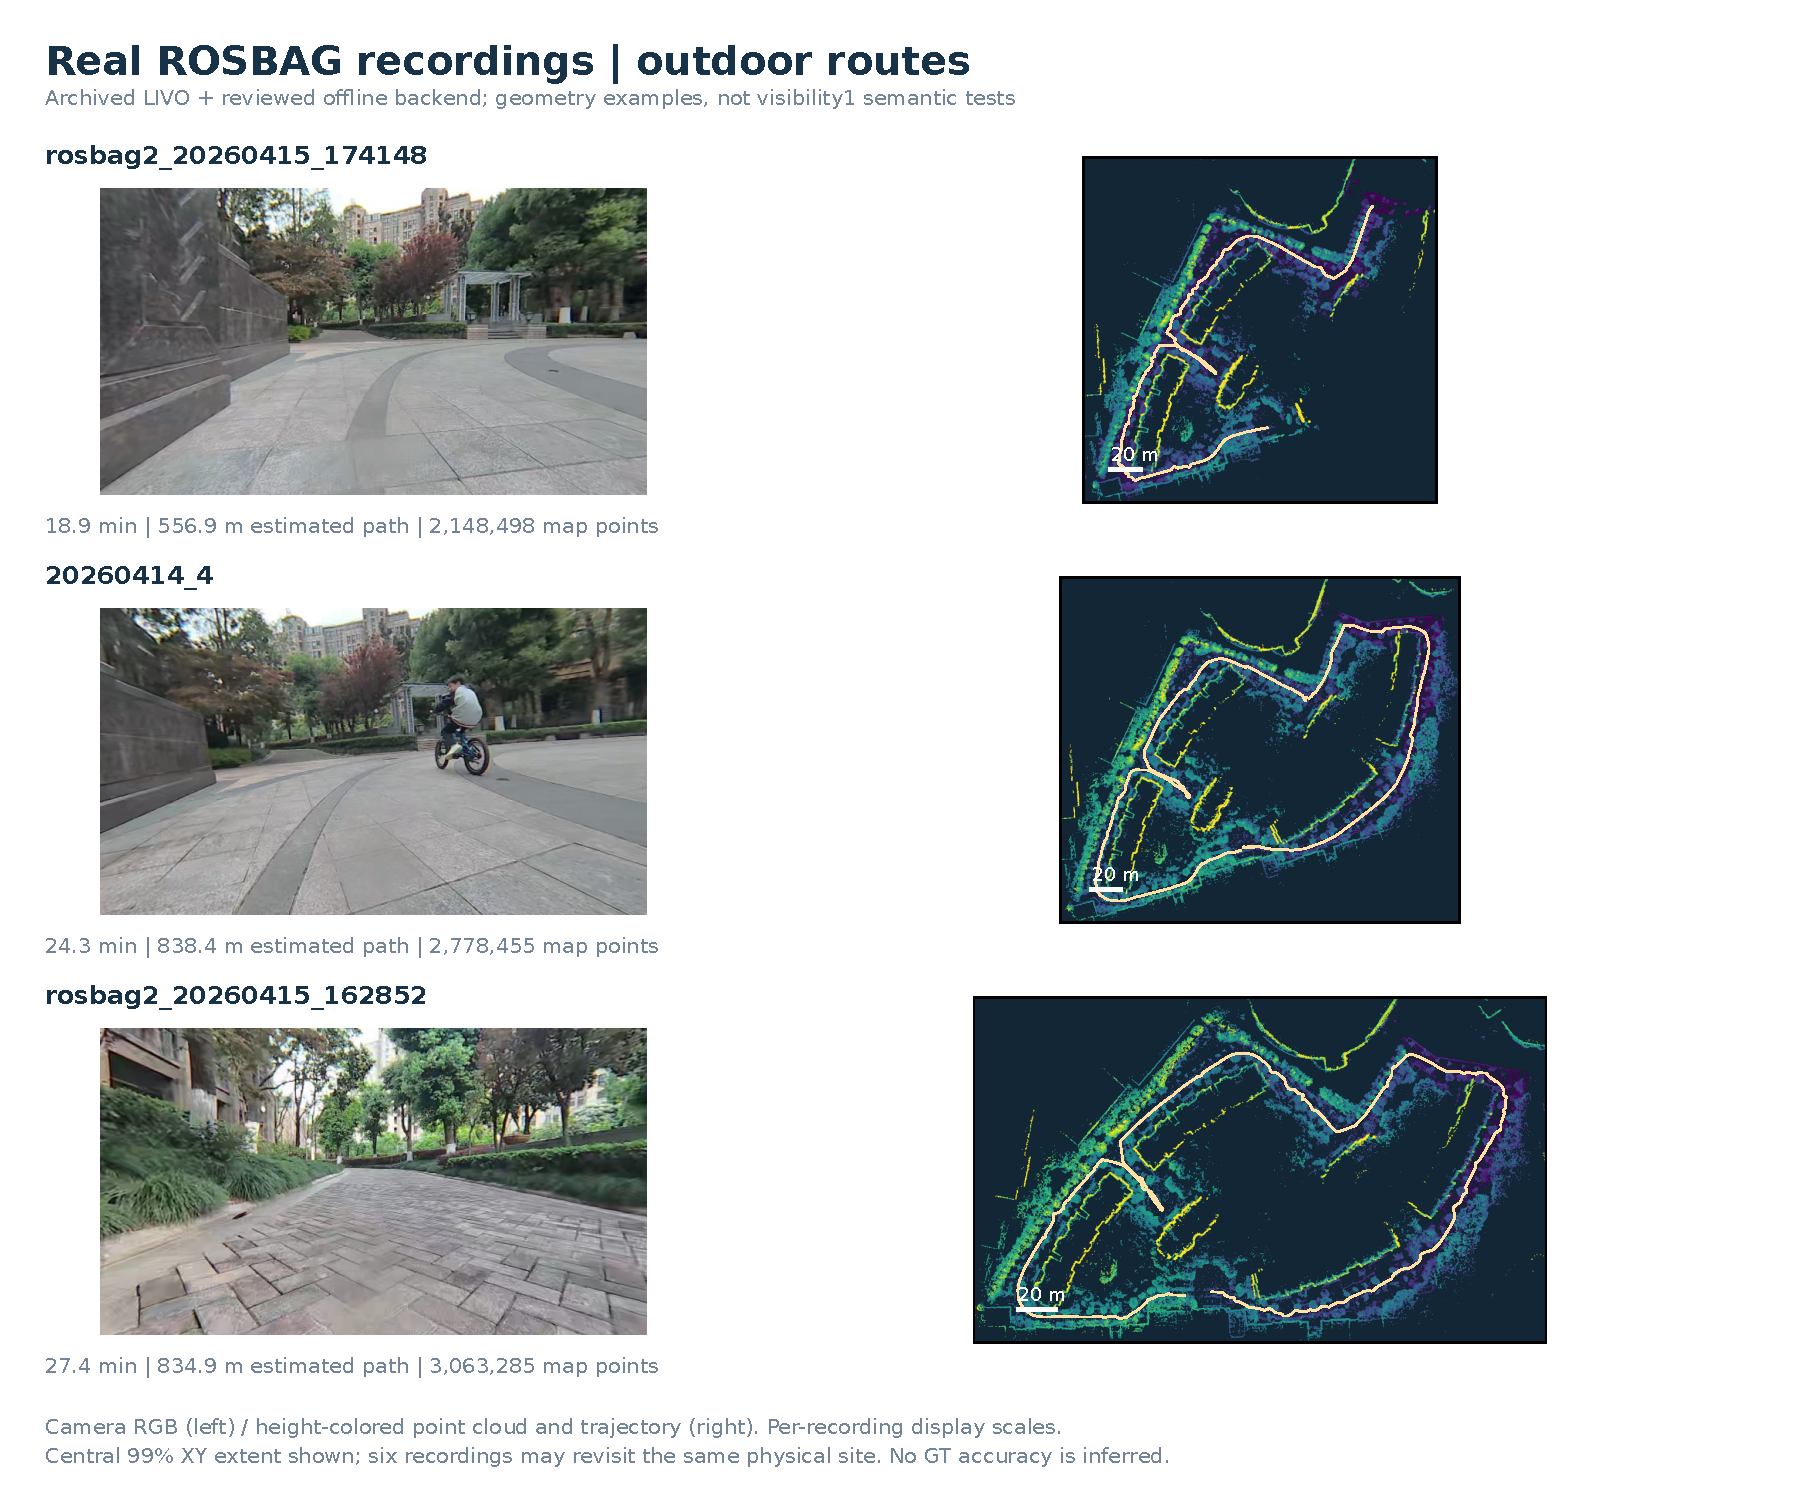
\includegraphics[width=.98\textwidth,height=.8\textheight,keepaspectratio]{rosbag_routes_2.pdf}
\caption{Three real outdoor recordings, including estimated paths of approximately $835$ and $838\,\mathrm m$. Map colors and display conventions match the preceding garage atlas. Spatial overlap between recordings is possible and does not establish independent-site coverage.}
\end{figure}
\clearpage

\section{Outdoor Landmarks and Measured Bounds}
\begin{figure}[h!]
\centering
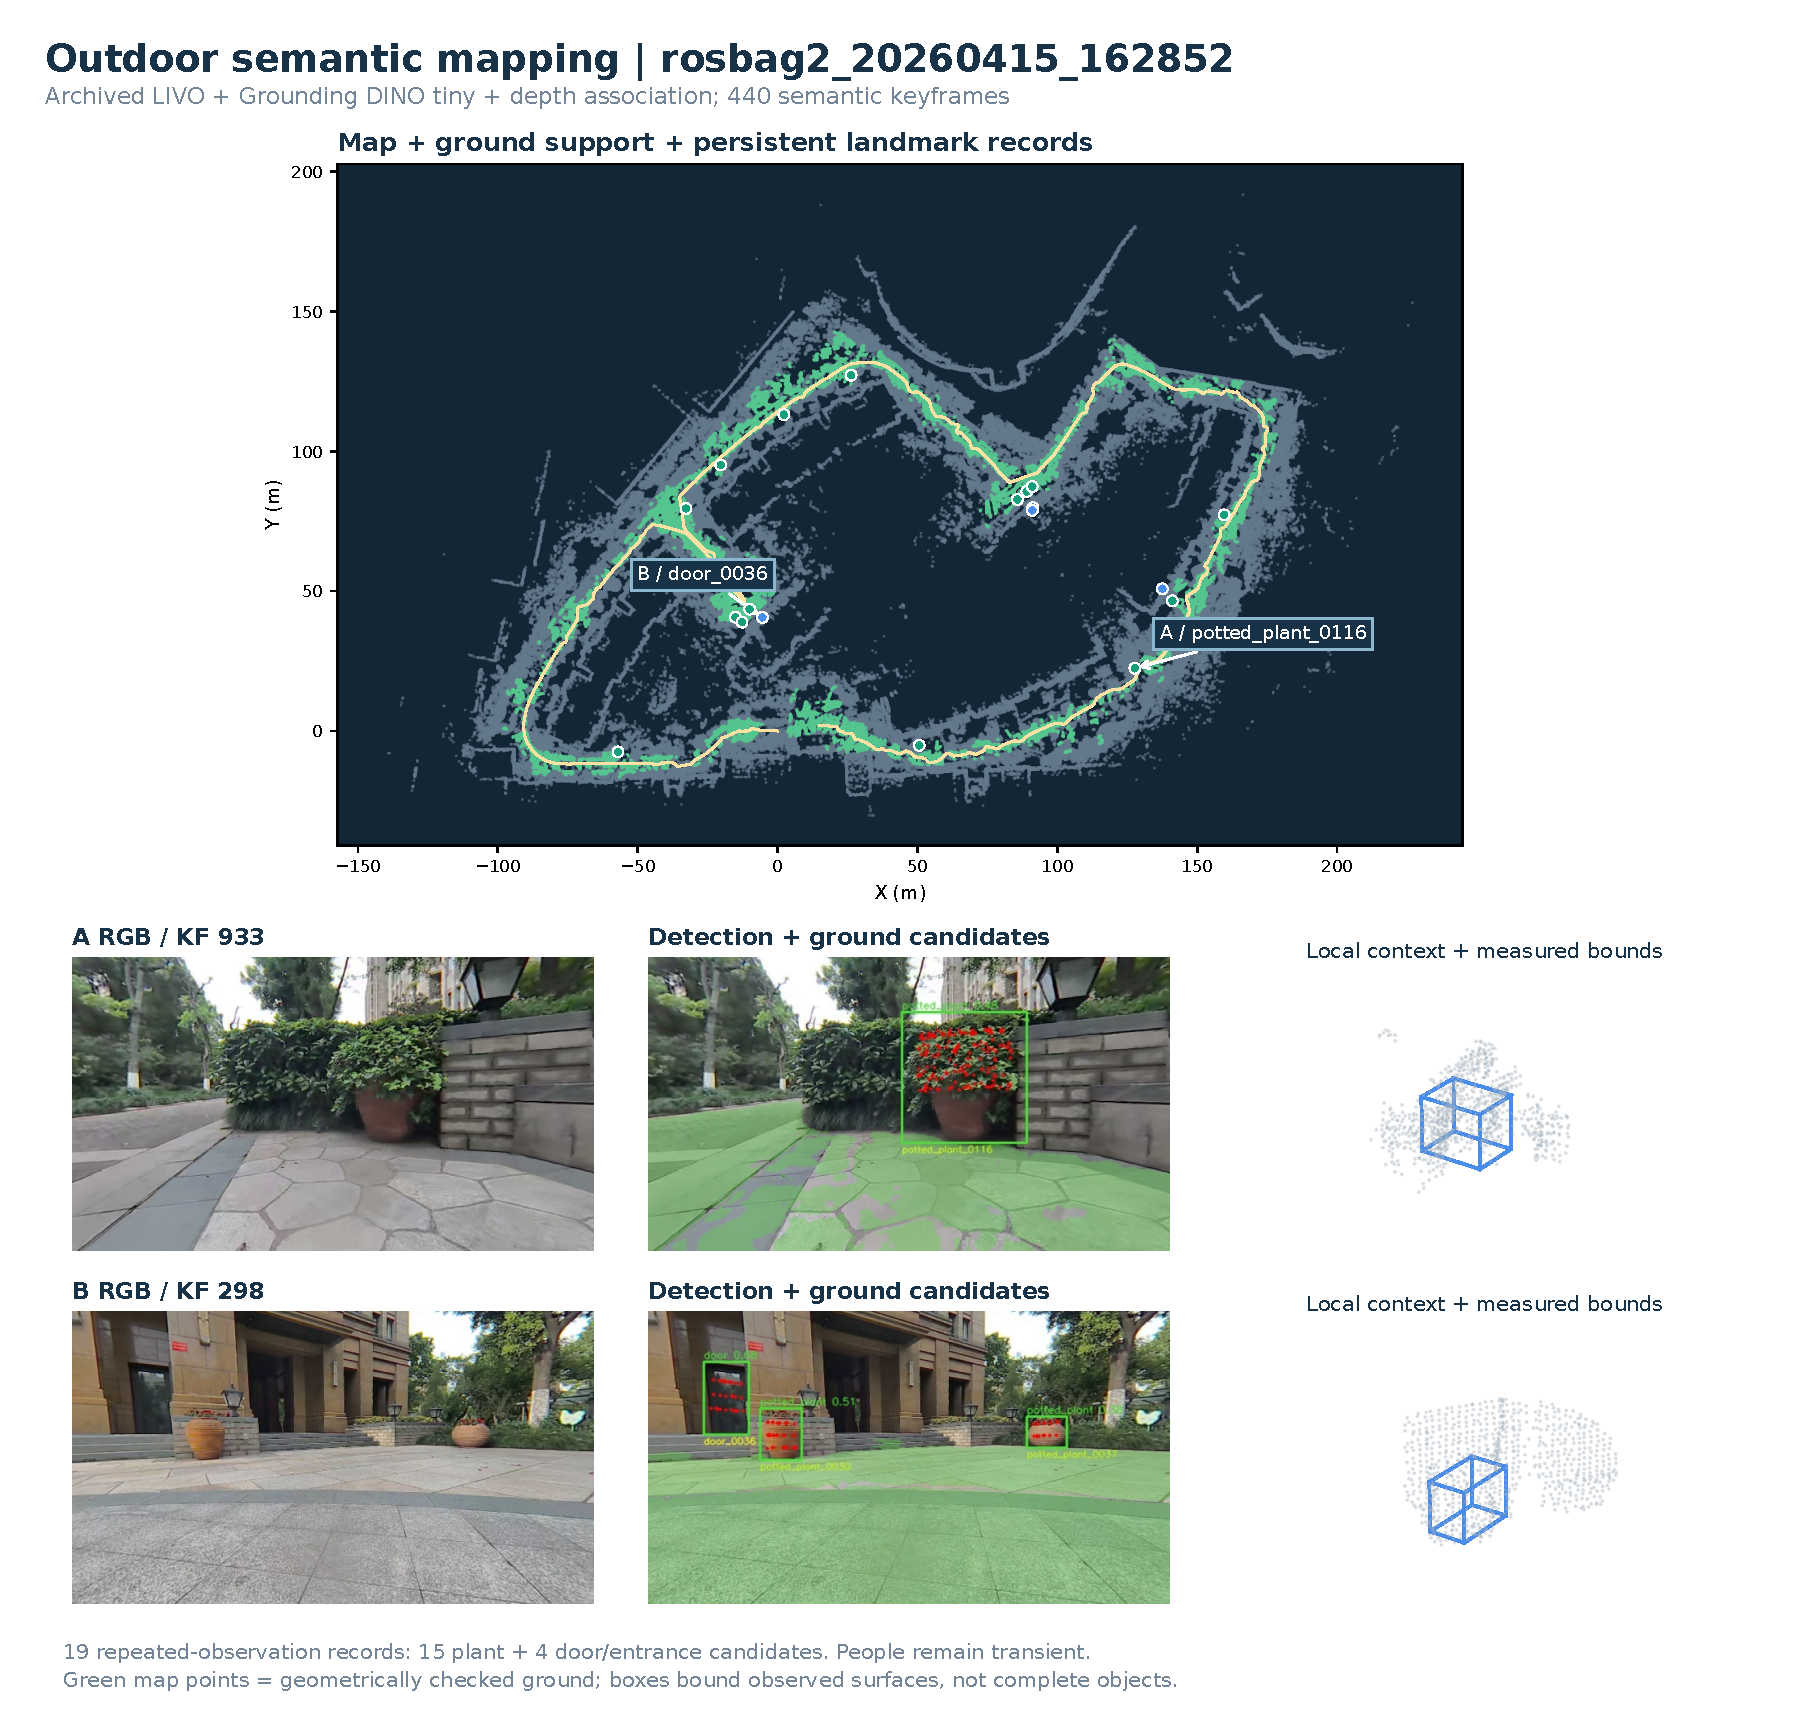
\includegraphics[width=.98\textwidth,height=.8\textheight,keepaspectratio]{rosbag_outdoor_semantics.pdf}
\caption{Archived outdoor semantic map, route, ground support, and two selected static records linked to their real image evidence and measured bounds. Gray points in the local 3D panels are surrounding map context rather than isolated object support. For each selected record, the largest observed image box is shown. Green map points are geometrically checked ground. Candidate categories and boxes are predictions, not ground-truth annotations.}
\end{figure}
\clearpage

\section{Ground Segmentation and Transient Observations}
\begin{figure}[h!]
\centering
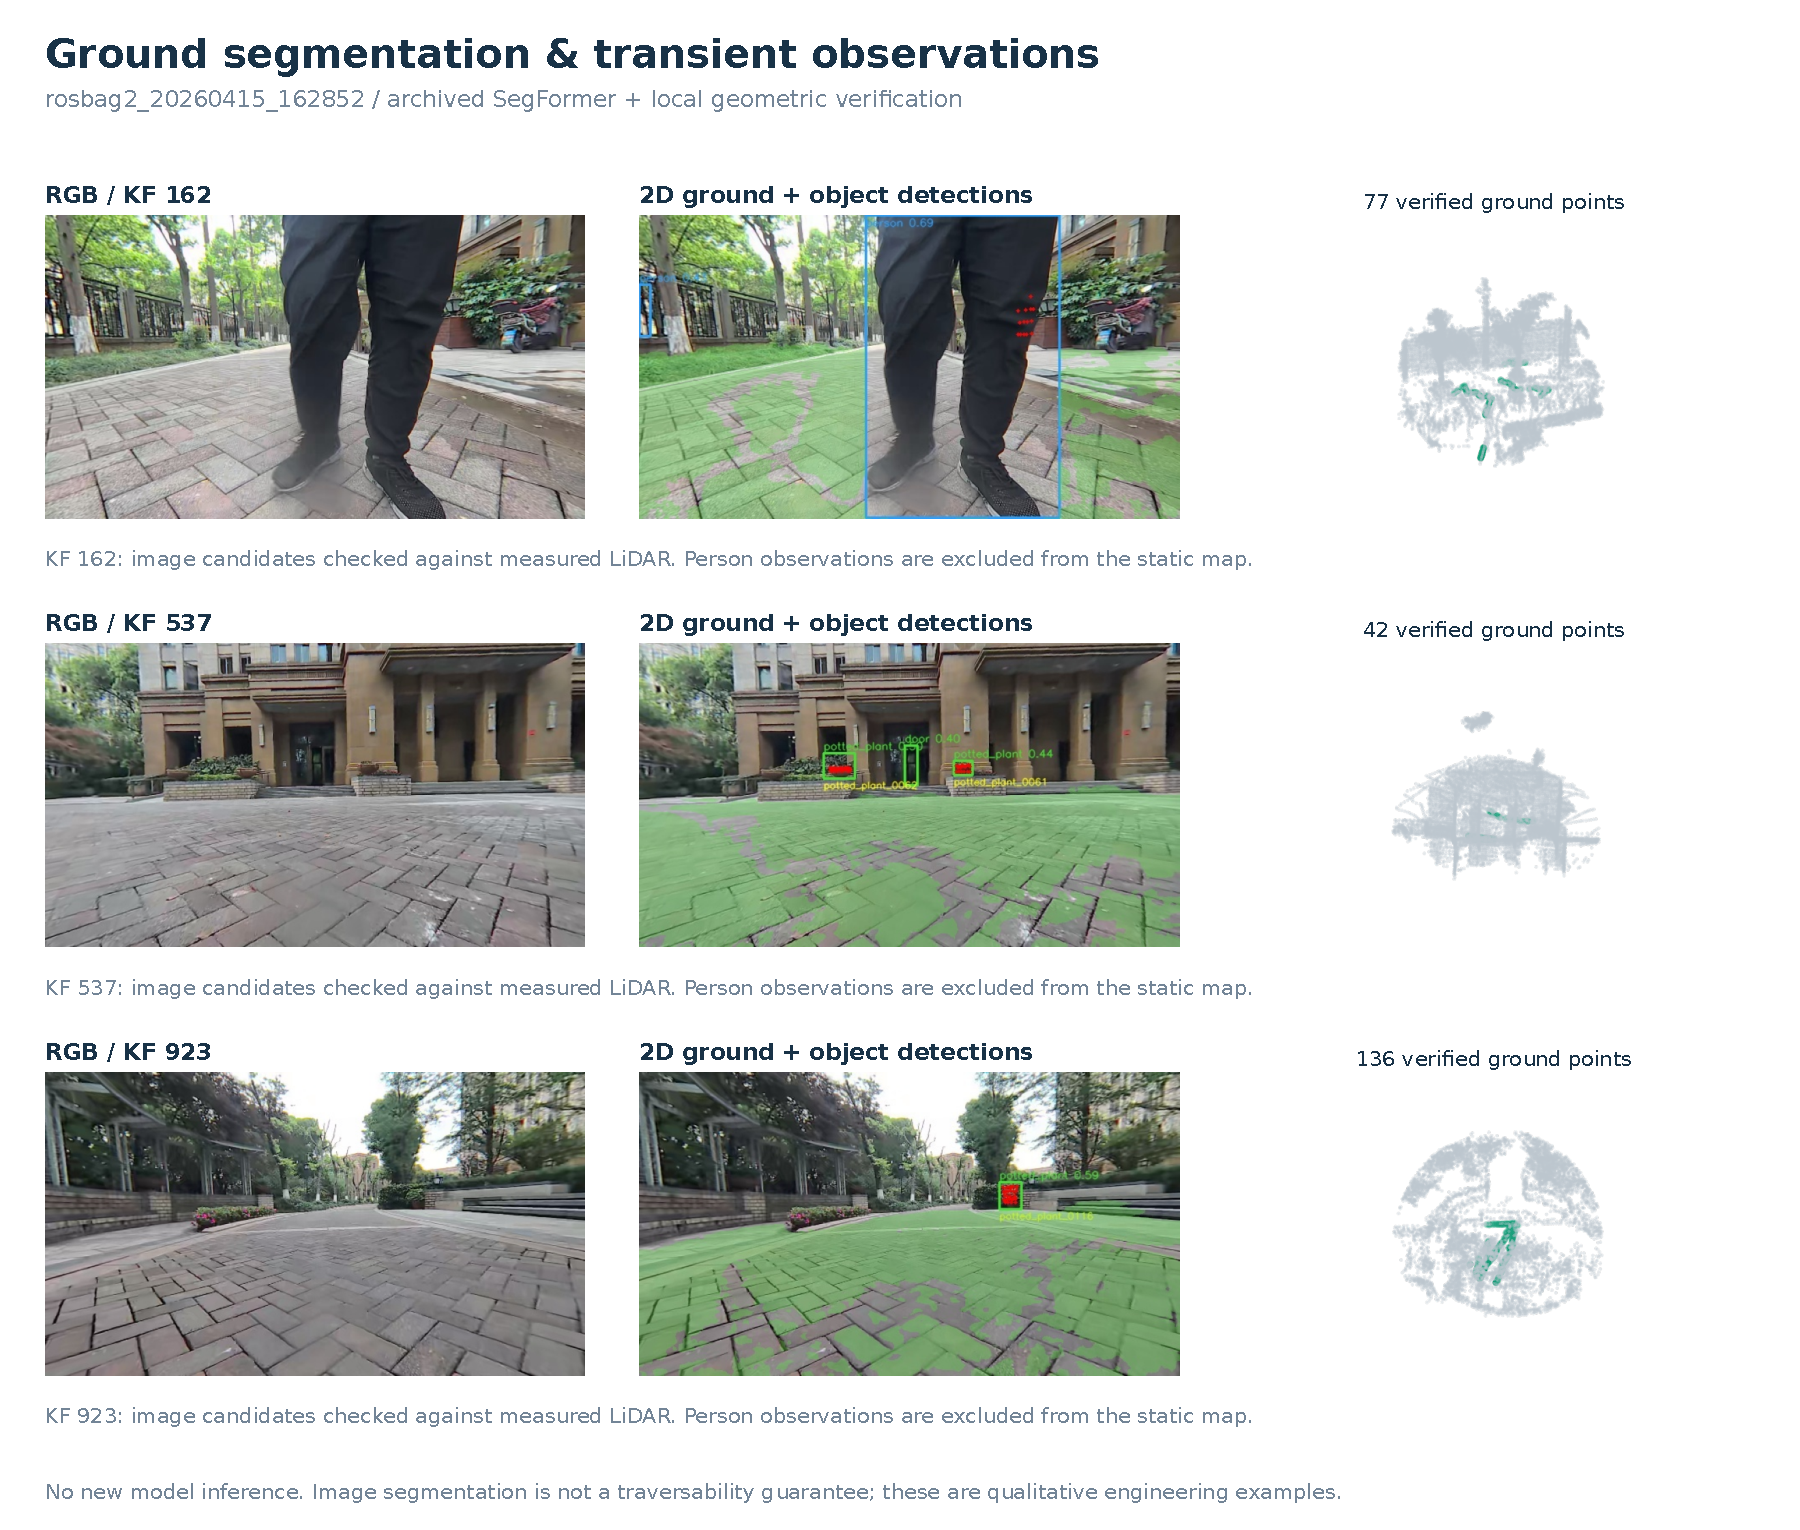
\includegraphics[width=.98\textwidth,height=.8\textheight,keepaspectratio]{rosbag_ground_details.pdf}
\caption{Three actual outdoor keyframes show raw RGB, image-level ground candidates and object detections, and corresponding verified LiDAR ground points in local map context. Image candidates and verified 3D points are distinct outputs. The selected frames have nonempty verified support; other frames may have image candidates but no accepted points. People are excluded from static landmarks. These qualitative examples are not a traversability guarantee or a quantitative ground-segmentation benchmark.}
\end{figure}
